% Provenance (never printed): old terminale S material on the early Earth (the
% primitive atmosphere and its outgassing, the first traces of life, the rise of
% oxygen read in the rocks: banded iron formations, red beds) and the faint young
% Sun. Owner (Sync 0/1): outgassing and primitive atmosphere, faint young Sun
% problem, stromatolite, Great Oxidation Event, banded iron formation, red beds.
% Recalled: age of the Earth (g12.07), zircons (g12.01), equilibrium temperature
% (g10.02), photosynthesis and cyanobacteria (biology), air composition, greenhouse
% gases as molecules and redox (chemistry). Figures: figdata/grade-12/early_earth.py.
\chapter{The Early Earth and Its Atmosphere}\label{ch:g12:early-earth}

In the Hamersley Ranges of north-western Australia, the walls of Dales Gorge
are striped like a layer cake: thin bands of red, grey and black rock. They
are a \omterm{def:g12:early-earth:bif}{banded iron formation}, laid down on a sea floor more than 2.5 billion
years ago.
The iron in them rusted in that sea, and to rust, it needed oxygen. This
chapter asks what the young Earth and its air were like, and how the rocks
record the moment oxygen appeared.
% ledger: dbca:karijini, earle:bif, photo:g12-dales-gorge

\begin{omfigure}
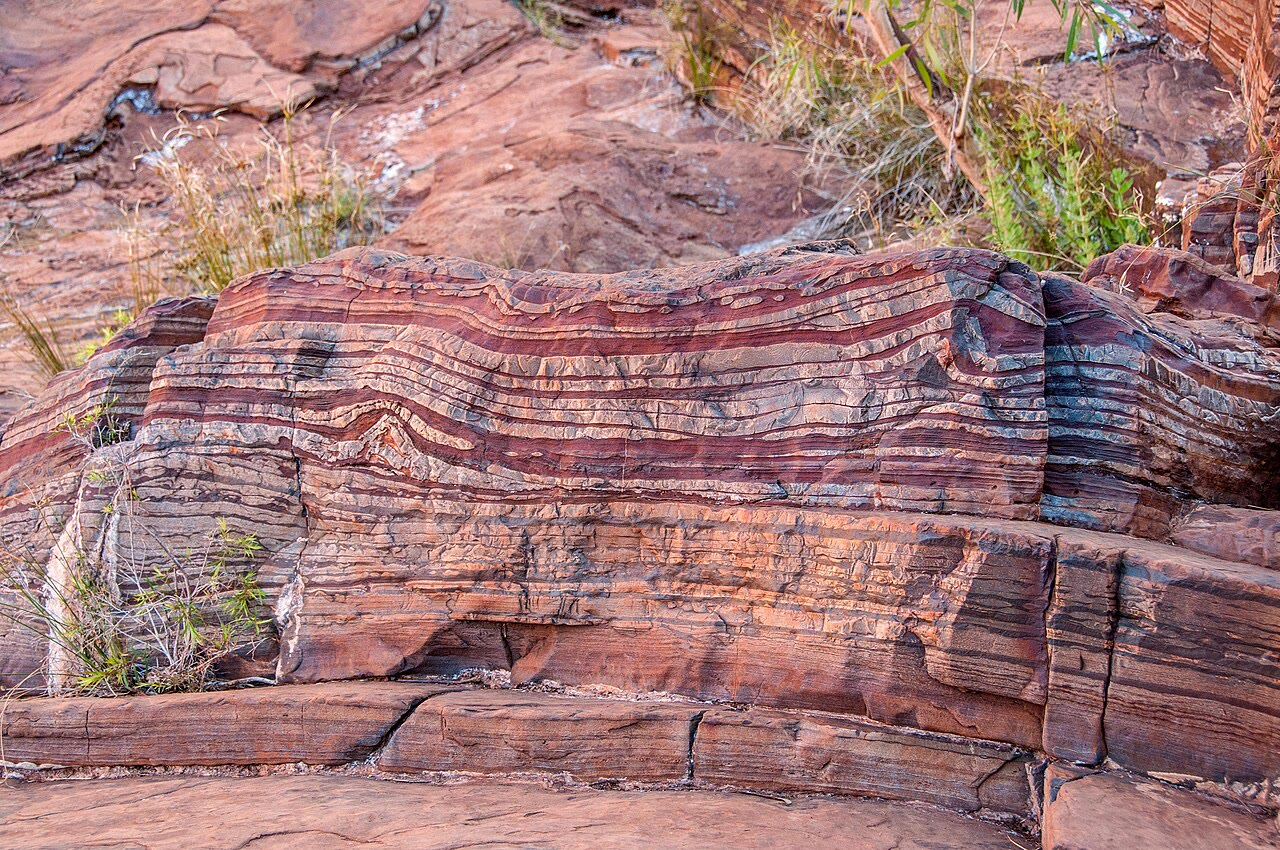
\includegraphics[width=0.72\linewidth]{images/book2/g12-dales-gorge-bif.jpg}

{\small \omterm{def:g12:early-earth:bif}{Banded iron formation} at Fortescue Falls, Dales Gorge, Karijini
National Park, Western Australia. Photograph Graeme Churchard, CC~BY~2.0
(Wikimedia Commons).}
\end{omfigure}

\begin{recall}
The Earth is 4.54 billion years old (\cref{ch:g12:age-of-the-earth}), and
zircons show that a crust existed 4.4 billion years ago
(\cref{ch:g12:continental-crust}). A planet's \omterm{def:g10:habitable-planet:equilibrium-temperature}{equilibrium temperature},
$T_{\mathrm{eq}} = \left(S(1-A)/(4\sigma)\right)^{1/4}$, is about \qty{255}{K}
for the Earth today (\cref{ch:g10:habitable-planet}). Today's dry air is
\qty{78}{\percent} nitrogen and \qty{21}{\percent} oxygen, and carbon dioxide and
methane are greenhouse gases; an element that takes up oxygen is oxidised (the
chemistry books). Plants, algae and cyanobacteria make their food by
photosynthesis, which releases oxygen (the biology books).
\end{recall}
% ledger: usgs:age-earth (Book 1 row), wilde01:zircon, earth:TSI, earth:albedo, air:N2, air:O2

\section{The young Earth}

The Earth grew by the accretion of smaller bodies. About 60 million years
after the Solar System began to form, a body perhaps the size of Mars struck
it, and the material flung into space formed the Moon. The young Earth was
hot and still partly molten. It cooled, and by about 4.4 billion years ago it
already had a crust and an ocean: zircons of that age carry the chemical mark
of liquid water.
% ledger: nasa:moon-formation, wilde01:zircon

\section{The primitive atmosphere}

\begin{definition}[Outgassing; primitive atmosphere]\label{def:g12:early-earth:primitive-atmosphere}
\emph{Outgassing}\index{outgassing} is the release, by volcanoes and through
the ground, of the gases dissolved in magma. The \emph{primitive
atmosphere}\index{primitive atmosphere} is the Earth's atmosphere before
living things changed it: built mostly by outgassing, it held nitrogen,
carbon dioxide and water vapour, more carbon dioxide than today, and almost
no free oxygen.
\end{definition}
% ledger: usgs:volcanic-gases (Book 1 row), holland06:stages (stage 1 anoxic), feulner12:fys (more carbon dioxide)

Volcanoes still show how such an atmosphere forms: as magma rises and the
pressure falls, its dissolved gases escape, by far the most abundant being
water vapour, then carbon dioxide. Nitrogen and carbon dioxide, the gases
that dominated the primitive air, are still the main nitrogen- and
carbon-bearing gases of volcanoes today. The water vapour condensed into the
ocean. Oxygen made up less than \qty{0.001}{\percent} of its level in today's
air.
% ledger: usgs:volcanic-gases (Book 1 row), pk02:anoxic

The young Sun shone less brightly than today. As it turns hydrogen into
helium in its core, the core contracts and heats up, and the Sun's power
slowly rises.

\begin{proposition}[The young Sun's luminosity]\label{prop:g12:early-earth:luminosity}
Calling $t_\odot$ the Sun's present age and $L_\odot$ its present
luminosity, its luminosity when it was $t$ years old was
\[
  L(t) = \frac{L_\odot}{1 + \frac{2}{5}\left(1 - t/t_\odot\right)} .
\]
\end{proposition}
% ledger: gough81:luminosity, connelly12:cai

This approximation of the computed models of the Sun is admitted here. At the
Sun's birth, $t = 0$, it gives $L = L_\odot/1.4 \approx 0.71\,L_\odot$:
the young Sun was about \qty{30}{\percent} dimmer.

\begin{example}[The Earth four billion years ago]\label{ex:g12:early-earth:young-sun}
Take $t_\odot = 4.567$ billion years. Four billion years ago the Sun was
0.567 billion years old, so $1 - t/t_\odot = 4/4.567 \approx 0.876$ and
$L \approx L_\odot/1.350 \approx 0.741\,L_\odot$. The sunlight reaching the
Earth was $0.741 \times 1361 \approx \qty{1008}{W/m^2}$. Keeping today's
\omterm{def:g10:earth-energy-budget:albedo}{albedo}, the \omterm{def:g10:habitable-planet:equilibrium-temperature}{equilibrium temperature} scales as the fourth root of the
sunlight: $255 \times 0.741^{1/4} \approx 255 \times 0.928 \approx
\qty{237}{K}$, about \qty{-36}{\celsius}.
\end{example}
% values: L_4Ga 0.7406, S_4Ga 1007.9, Teq_today 255.1, Teq_4Ga 236.7 (early_earth.py)

\begin{omfigure}
\begin{tikzpicture}
\begin{axis}[omrecord, scale only axis, width=0.66\linewidth, height=4.6cm,
  xmin=0, xmax=4.6, ymin=225, ymax=295, x dir=reverse, axis y line*=left,
  xlabel={time before present (billion years)}, ylabel={temperature (K)},
  xtick={0,0.5,...,4.5}, x tick label style={/pgf/number format/.cd, fixed, precision=1}]
% computed in figdata/grade-12/early_earth.py; ledger: gough81:luminosity, earth:TSI, earth:albedo, earth:Tsurf
\addplot[omDef, line width=1.2pt] table[x=t_Ga, y=Teq] {figdata/out/grade-12-early_earth-sun.dat};
\addplot[omThm, densely dashed, domain=0:4.6, samples=2] {273.15};
\addplot[black!60, densely dotted, domain=0:4.6, samples=2] {288};
\coordinate (teq) at (axis cs:2.6,239);
\coordinate (frz) at (axis cs:2.3,274);
\coordinate (sfc) at (axis cs:2.3,289);
\end{axis}
\begin{axis}[omrecord, scale only axis, width=0.66\linewidth, height=4.6cm,
  xmin=0, xmax=4.6, ymin=0.65, ymax=1.05, x dir=reverse, axis y line*=right, axis x line=none,
  ylabel={Sun's luminosity ($L_\odot$)}, ymajorgrids=false, xmajorgrids=false,
  y tick label style={/pgf/number format/.cd, fixed, fixed zerofill, precision=2}]
\addplot[omProp, line width=0.9pt, densely dashdotted] table[x=t_Ga, y=L] {figdata/out/grade-12-early_earth-sun.dat};
\coordinate (lum) at (axis cs:1.7,0.86);
\end{axis}
\node[font=\scriptsize, text=omDef, anchor=north] at (teq) {equilibrium temperature};
\node[font=\scriptsize, text=omThm, anchor=south] at (frz) {water freezes, \qty{273}{K}};
\node[font=\scriptsize, text=black!70, anchor=south] at (sfc) {mean surface today, \qty{288}{K}};
\node[font=\scriptsize, text=omProp, anchor=north west] at (lum) {luminosity (right scale)};
\end{tikzpicture}

{\small The faint young Sun: its luminosity (right scale) and the Earth's
\omterm{def:g10:habitable-planet:equilibrium-temperature}{equilibrium temperature} with today's \omterm{def:g10:earth-energy-budget:albedo}{albedo} (left scale), back to the birth
of the Sun. Computed from Gough (1981) with today's sunlight and \omterm{def:g10:earth-energy-budget:albedo}{albedo}.}
\end{omfigure}

\begin{definition}[Faint young Sun problem]\label{def:g12:early-earth:faint-young-sun}
The \emph{faint young Sun problem}\index{faint young Sun problem} is the
contradiction between the dimmer Sun of the Earth's first billions of years,
under which the Earth with today's atmosphere would have frozen, and the
rocks, which show that liquid water was present.
\end{definition}
% ledger: feulner12:fys

The problem was made widely known in 1972 by Carl Sagan and George Mullen,
who proposed a stronger greenhouse effect as the answer. Most of the answers
studied since call on more greenhouse gases in the \omterm{def:g12:early-earth:primitive-atmosphere}{primitive atmosphere}:
much more carbon dioxide than today, methane made by early microbes, or
both. In one classic calculation, about a tenth of a bar of carbon dioxide,
with a little methane, keeps the young Earth as warm as today; without the
methane, about three times more is needed. The problem is not yet regarded
as solved.
% ledger: feulner12:fys

\section{Life and oxygen}

The fossil record of \omterm{def:g12:early-earth:stromatolite}{stromatolites} covers almost \num{3500} million years:
they are among the oldest signs of life.

\begin{definition}[Stromatolite]\label{def:g12:early-earth:stromatolite}
A \emph{stromatolite}\index{stromatolite} is a layered mound built in
shallow water by a mat of microbes, mainly cyanobacteria, which trap and
bind grains of sediment and make carbonate grow, layer upon layer.
\end{definition}
% ledger: noffke13:stromatolites

Fossil \omterm{def:g12:early-earth:stromatolite}{stromatolites} \num{3430} million years old are found in the Strelley
Pool Chert of the Pilbara, in Western Australia. Living ones grow today in
the very salty water of Hamelin Pool in Shark Bay, twice as salty as usual
sea water, where they are the best-known modern example.
% ledger: allwood06:spc, noffke13:stromatolites, dbca:hamelin

\begin{omfigure}
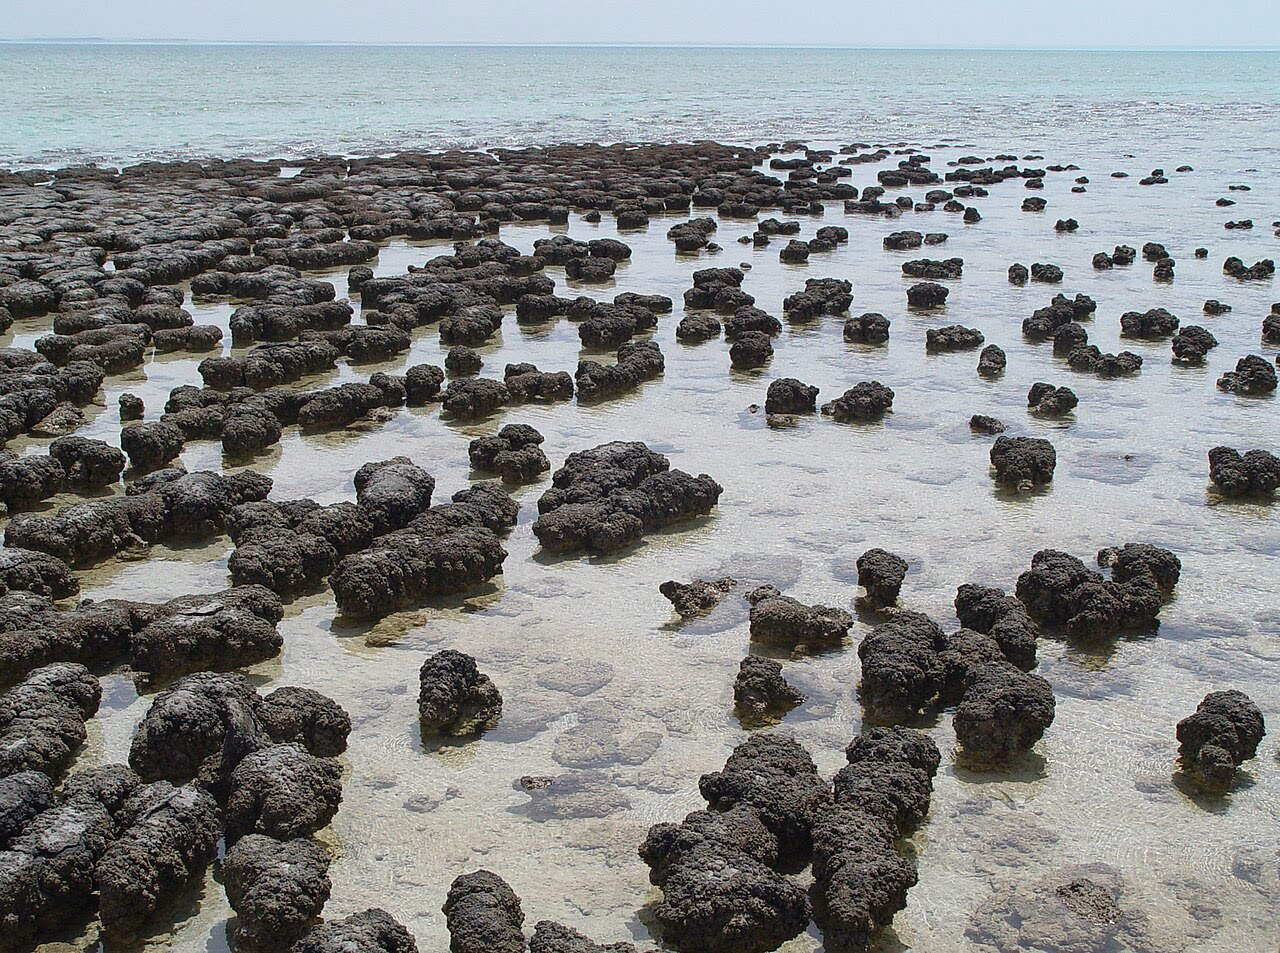
\includegraphics[width=0.6\linewidth]{images/book2/g12-shark-bay-stromatolites.jpg}

{\small Living \omterm{def:g12:early-earth:stromatolite}{stromatolites} in Hamelin Pool, Shark Bay, Western Australia.
Photograph Paul Harrison, CC~BY-SA~3.0 (Wikimedia Commons).}
\end{omfigure}
% ledger: photo:g12-shark-bay

The cyanobacteria brought something new: photosynthesis that releases
oxygen. But for a long time the oxygen they made did not stay in the air. It
was used up as fast as it was made: by the iron dissolved in the sea, by
sulfur and by methane.

\section{The rise of oxygen}

Before oxygen, iron could travel dissolved in sea water as the ion
\ce{Fe^2+}. Oxygen turns it into iron(III), which does not dissolve: it falls
to the floor as a rusty sediment.

\begin{proposition}[Iron takes up oxygen]\label{prop:g12:early-earth:iron}
Dissolved iron(II) is oxidised by oxygen in water into iron(III) hydroxide,
which precipitates:
\[
  \ce{4Fe^2+ + O2 + 10H2O -> 4Fe(OH)3 + 8H+} .
\]
Each molecule of oxygen removes four ions of dissolved iron; as long as
dissolved iron remains, the oxygen made is used up.
\end{proposition}
% ledger: earle:bif (ferrous iron oxidised to insoluble ferric iron)

\begin{proof}
Check the balance. Iron: 4 on each side. Oxygen: $2 + 10 = 12$ on the left,
$4 \times 3 = 12$ on the right. Hydrogen: $20$ on the left, $4 \times 3 + 8 =
20$ on the right. Charge: $4 \times (+2) = +8$ on the left, $8 \times (+1) =
+8$ on the right.
\end{proof}

\begin{definition}[Banded iron formation]\label{def:g12:early-earth:bif}
A \emph{banded iron formation}\index{banded iron formation} is a
sedimentary rock of thin alternating layers of iron oxides, such as
hematite, and of chert, a fine-grained silica poor in iron. Almost all are
older than 1.8 billion years.
\end{definition}
% ledger: earle:bif, holland06:stages

\omterm{def:g12:early-earth:bif}{Banded iron formations} need two waters at once: a \omterm{def:g10:layered-ocean:thermocline}{deep ocean} without oxygen,
which carries dissolved iron, and a shallow, sunlit sea where cyanobacteria
make oxygen and the iron precipitates. They are common in rocks from 2.4 to
1.8 billion years old, and those of the Hamersley Ranges are older still.
\omterm{def:g12:early-earth:bif}{Banded iron formations} are a common ore of iron.
% ledger: earle:bif, holland06:stages (Archean BIF, Hamersley), dbca:karijini

\begin{omfigure}
\begin{tikzpicture}[x=1cm, y=1cm, font=\scriptsize]
  % sea and floor
  \fill[omSea] (0,0) rectangle (11,4);
  \fill[omSea!45!white] (0,2.9) rectangle (11,4);
  \draw[omDef!60, line width=0.4pt, densely dashed] (0,2.9) -- (11,2.9);
  \node[anchor=north east, text=omDef] at (10.9,3.95) {sunlit surface water};
  \node[anchor=south east, text=omDef, align=right] at (10.9,0.12) {deep water\\without oxygen,\\rich in \ce{Fe^2+}};
  % floor with layers
  \foreach \i/\c in {0/red!55!black, 1/black!20, 2/red!55!black, 3/black!20, 4/red!55!black, 5/black!20} {
    \fill[\c] (0,-0.12*\i) rectangle (11,-0.12*\i-0.12);
  }
  \draw[black!60] (0,0) -- (11,0);
  \node[anchor=west] at (11.1,-0.12) {iron oxide};
  \node[anchor=west] at (11.1,-0.36) {chert};
  \draw[black!50, line width=0.3pt] (11.05,-0.06) -- (10.6,-0.06);
  \draw[black!50, line width=0.3pt] (11.05,-0.30) -- (10.6,-0.30);
  % upwelling iron
  \foreach \x in {0.5,1.0,1.5} {
    \draw[-{Stealth}, omDef, line width=0.8pt] (\x,0.4) .. controls (\x+0.4,1.5) and (\x+0.6,2.2) .. (\x+0.9,2.85);
  }
  \node[text=omDef, anchor=west] at (2.3,1.3) {\ce{Fe^2+} rises};
  % cyanobacteria and oxygen
  \foreach \x in {3.8,4.4,5.0,5.6,6.2} {\fill[green!45!black] (\x,3.35) circle (0.07);}
  \node[anchor=south, text=green!35!black] at (5.0,3.47) {cyanobacteria make \ce{O2}};
  % reaction
  \node[draw=black!40, fill=white, rounded corners=2pt, inner sep=2pt] at (5.4,2.45) {\ce{4Fe^2+ + O2 + 10H2O -> 4Fe(OH)3 + 8H+}};
  % falling rust
  \foreach \x/\y in {4.6/1.9, 5.0/1.5, 5.5/1.8, 5.9/1.2, 4.3/1.1, 5.2/0.7, 6.1/0.6} {\fill[red!60!black] (\x,\y) circle (0.06);}
  \draw[-{Stealth}, red!60!black, line width=0.6pt] (6.6,2.1) -- (6.6,0.25);
  \node[anchor=west, text=red!60!black, align=left] at (6.7,1.75) {iron(III) settles\\as a rusty layer};
\end{tikzpicture}

{\small How a \omterm{def:g12:early-earth:bif}{banded iron formation} forms (schematic, not to scale): iron
dissolved in the deep water, which holds no oxygen, rises into the sunlit
sea, where the oxygen made by cyanobacteria turns it into iron(III), which
settles. Layers rich in iron alternate with layers of chert.}
\end{omfigure}

Then oxygen began to stay in the air.

\begin{definition}[Great Oxidation Event]\label{def:g12:early-earth:goe}
The \emph{Great Oxidation Event}\index{Great Oxidation Event} is the
interval, from about \num{2.46} to about \num{2.06} billion years ago, during
which free oxygen first built up in the Earth's atmosphere and shallow seas,
reaching perhaps a tenth of its present level.
\end{definition}
% ledger: gumsley17:goe, holland06:stages (0.02-0.04 atm, about a tenth of 0.21)

The evidence is in the rocks. Some minerals, pyrite and uraninite among
them, are destroyed by oxygen; yet grains of them, rolled by rivers, are
found in old sediments, and grains of pyrite are missing from those laid
down after the rise of oxygen. Sulfur isotopes in rocks older than about 2.45 billion years carry a
signature that only an air with less than a hundred-thousandth of today's
oxygen can leave; by 2.09 billion years ago it has gone. And on land appeared
\omterm{def:g12:early-earth:red-beds}{red beds}.
% ledger: kasting25:indicators, pk02:anoxic, farquhar00:sulfur

\begin{definition}[Red beds]\label{def:g12:early-earth:red-beds}
\emph{Red beds}\index{red beds} are sedimentary rocks --- sandstones,
siltstones, shales --- coloured red by a coating of iron(III) oxide,
hematite, on their grains. They form only where there is oxygen enough to
oxidise iron.
\end{definition}
% ledger: kasting25:indicators (redbeds an oxygen indicator)

\begin{omfigure}
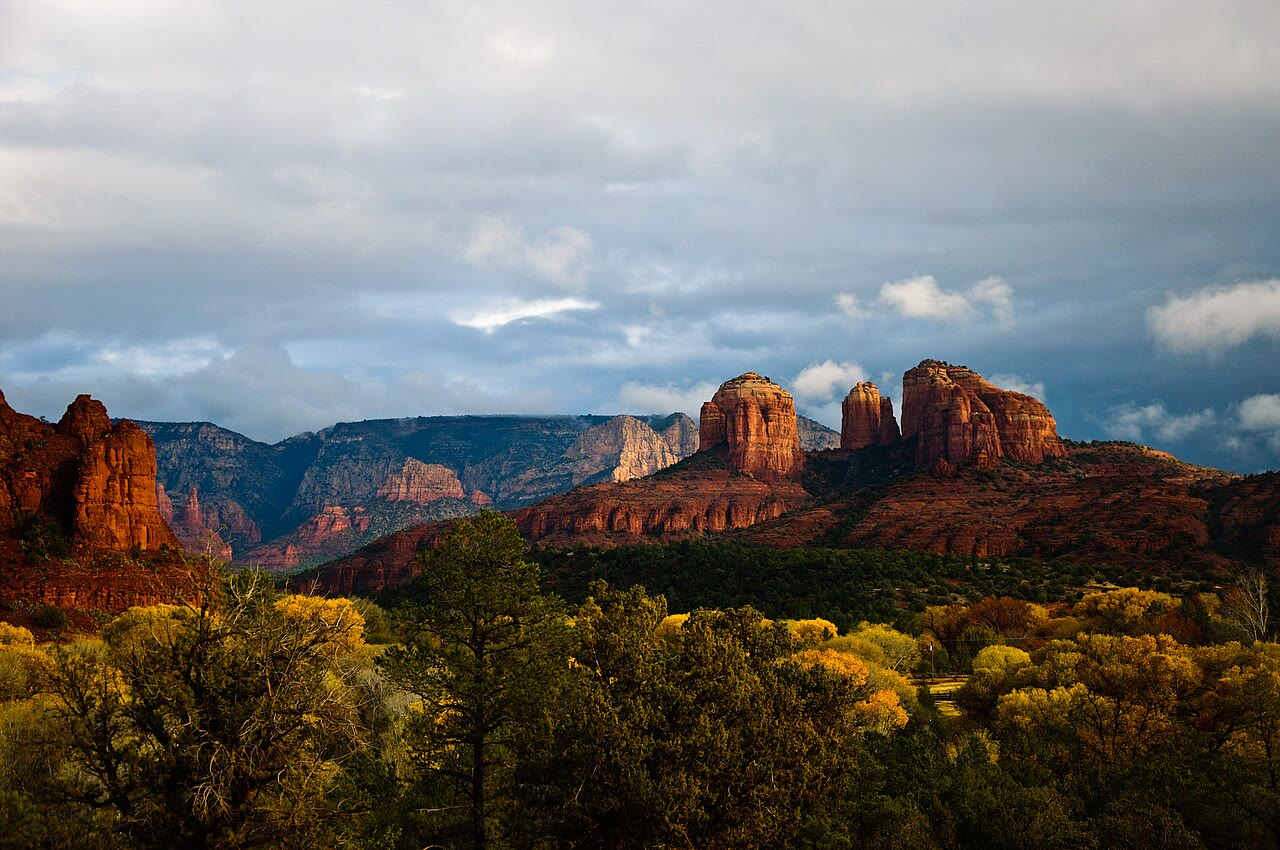
\includegraphics[width=0.66\linewidth]{images/book2/g12-sedona-red-beds.jpg}

{\small \omterm{def:g12:early-earth:red-beds}{Red beds}: Cathedral Rock near Sedona, Arizona, built of Permian red
sandstones. Photograph Wendy from Pennsylvania, CC~BY-SA~2.0 (Wikimedia
Commons).}
\end{omfigure}
% ledger: photo:g12-sedona, azgs:cathedral (Permian Schnebly Hill Sandstone)

The formation of \omterm{def:g12:early-earth:bif}{banded iron formations} essentially stopped after 1.8 billion
years ago: by then the \omterm{def:g10:layered-ocean:thermocline}{deep ocean} too had enough oxygen to stop carrying
iron. Over the next billion years oxygen changed little; after 0.85 billion
years ago it built up again, towards today's \qty{21}{\percent}.
% ledger: earle:bif, holland06:stages

\begin{method}[Reading a geological timeline]\label{met:g12:early-earth:timeline}
\begin{enumerate}
  \item Find which way time runs on the axis, and its unit (millions or
        billions of years before present).
  \item Locate the eons on the coloured band, and read their limits.
  \item For each event, read its date, or the interval during which it
        happened, and say what record dates it (a mineral, a fossil, a rock).
  \item Compute durations by subtraction, and compare them with the \omterm{def:g12:age-of-the-earth:age}{age of
        the Earth}.
  \item Check the order: an effect must not come before its cause.
\end{enumerate}
\end{method}

\begin{omfigure}
\begin{tikzpicture}
\begin{axis}[omrecord, width=0.82\linewidth, height=6.2cm, ymode=log, xmin=0, xmax=4.6, ymin=1e-7, ymax=5,
  x dir=reverse, xlabel={time before present (billion years)}, ylabel={oxygen in the air (today $=1$)},
  xtick={0,0.5,...,4.5}, x tick label style={/pgf/number format/.cd, fixed, precision=1},
  ytick={1e-6,1e-4,1e-2,1}, ymajorgrids=true, xmajorgrids=false, clip=false]
% computed in figdata/grade-12/early_earth.py (schematic through the sourced bounds); ledger: holland06:stages, pk02:anoxic, gumsley17:goe, ics:base.Hadean, ics:base.Archean, ics:base.Proterozoic, ics:base.Paleozoic
\fill[omThm!12] (axis cs:2.46,1e-7) rectangle (axis cs:2.06,5);
\addplot[black, line width=1.2pt] table[x=t_Ga, y=pal] {figdata/out/grade-12-early_earth-oxygen.dat};
% eon band (ICS colours), below the axis
\fill[icsHadean] (axis cs:4.567,1.5e-7) rectangle (axis cs:4.031,4e-7);
\fill[icsArchean] (axis cs:4.031,1.5e-7) rectangle (axis cs:2.5,4e-7);
\fill[icsProterozoic] (axis cs:2.5,1.5e-7) rectangle (axis cs:0.5388,4e-7);
\fill[icsPhanerozoic] (axis cs:0.5388,1.5e-7) rectangle (axis cs:0,4e-7);
\node[font=\tiny, text=white] at (axis cs:4.30,2.45e-7) {Hadean};
\node[font=\tiny, text=white] at (axis cs:3.27,2.45e-7) {Archean};
\node[font=\tiny, text=white] at (axis cs:1.52,2.45e-7) {Proterozoic};
% events
\draw[omDef, line width=0.6pt] (axis cs:4.4,4e-7) -- (axis cs:4.4,3e-3);
\node[font=\scriptsize, text=omDef, anchor=south west] at (axis cs:4.4,3e-3) {zircons, water};
\draw[omMeth, line width=0.6pt] (axis cs:3.43,4e-7) -- (axis cs:3.43,1.2e-6);
\node[font=\scriptsize, text=omMeth, anchor=south] at (axis cs:3.43,1.2e-6) {first stromatolites};
\draw[red!60!black, line width=3pt] (axis cs:2.4,3e-6) -- (axis cs:1.8,3e-6);
\node[font=\scriptsize, text=red!60!black, anchor=north] at (axis cs:2.16,2.4e-6) {banded iron formations};
\node[font=\scriptsize, text=omThm, anchor=south, align=center] at (axis cs:2.26,1.2) {Great Oxidation\\Event};
\node[font=\scriptsize, anchor=south] at (axis cs:3.2,1.3e-5) {less than $10^{-5}$ of today};
\node[font=\scriptsize, anchor=south] at (axis cs:1.4,0.12) {about a tenth};
\end{axis}
\end{tikzpicture}

{\small Oxygen in the air through time (schematic, logarithmic scale): the
curve joins the measured bounds and hides the ups and downs of the real
record. The shaded interval is the \omterm{def:g12:early-earth:goe}{Great Oxidation Event}; the red bar marks
the time when \omterm{def:g12:early-earth:bif}{banded iron formations} were common, 2.4 to 1.8 billion years
ago. Eons from the International
Chronostratigraphic Chart.}
\end{omfigure}

\section{Exercises}

\begin{exercise}[$\star$]\label{exo:g12:early-earth:1}
Give the word: (a) the release of gases dissolved in magma; (b) a layered
mound built by a microbial mat; (c) a rock of alternating iron-oxide and
chert layers; (d) sedimentary rocks coloured by hematite; (e) the interval
when oxygen first built up in the air.
\end{exercise}

\begin{exercise}[$\star$]\label{exo:g12:early-earth:2}
Put in order, from the oldest: the end of most \omterm{def:g12:early-earth:bif}{banded iron formations}; the
first \omterm{def:g12:early-earth:stromatolite}{stromatolites} of the Pilbara; zircons that show liquid water; the
Hamersley \omterm{def:g12:early-earth:bif}{banded iron formations}; the end of the \omterm{def:g12:early-earth:goe}{Great Oxidation Event}.
\end{exercise}

\begin{exercise}[$\star$]\label{exo:g12:early-earth:3}
Using the luminosity law, compute the Sun's luminosity at its birth, as a
fraction of today's. By what percentage was it dimmer?
\end{exercise}

\begin{exercise}[$\star$]\label{exo:g12:early-earth:4}
Grains of pyrite rolled by rivers are found in old sediments, but not in
those laid down after the rise of oxygen. What does this tell you about the
air at the time of the old sediments? Why?
\end{exercise}

\begin{exercise}[$\star$]\label{exo:g12:early-earth:5}
Name the two most abundant gases released by volcanoes, and say what became
of each in the young Earth.
\end{exercise}

\begin{exercise}[$\star\star$]\label{exo:g12:early-earth:6}
Compute the Sun's luminosity and the Earth's \omterm{def:g10:habitable-planet:equilibrium-temperature}{equilibrium temperature} (today
\qty{255}{K}, \omterm{def:g10:earth-energy-budget:albedo}{albedo} unchanged) 3 billion years ago and 2.45 billion years
ago, taking $t_\odot = 4.567$ billion years.
\end{exercise}

\begin{exercise}[$\star\star$]\label{exo:g12:early-earth:7}
How much oxygen is needed to precipitate \qty{1}{kg} of dissolved iron as
iron(III) hydroxide? (Molar masses: iron \qty{55.85}{g/mol}, oxygen
\qty{16.00}{g/mol}.)
\end{exercise}

\begin{exercise}[$\star\star$]\label{exo:g12:early-earth:8}
Using the timeline, (1) how long did the \omterm{def:g12:early-earth:goe}{Great Oxidation Event} last? (2)
For what fraction of the Earth's history was there almost no oxygen in the
air? (3) How long after the first \omterm{def:g12:early-earth:stromatolite}{stromatolites} did oxygen start to build up?
\end{exercise}

\begin{exercise}[$\star\star$]\label{exo:g12:early-earth:9}
A \omterm{def:g12:early-earth:bif}{banded iron formation} and a red bed both contain iron(III) oxide. What
does each tell you about oxygen, and where: in the deep sea, in the shallow
sea, in the air?
\end{exercise}

\begin{exercise}[$\star\star$]\label{exo:g12:early-earth:10}
Where can living \omterm{def:g12:early-earth:stromatolite}{stromatolites} be seen today? What is special about the
water there, and how does a \omterm{def:g12:early-earth:stromatolite}{stromatolite} grow layer upon layer?
\end{exercise}

\begin{exercise}[$\star\star$]\label{exo:g12:early-earth:11}
Oxygen is \qty{21}{\percent} of today's air. What percentage was it when it
was (1) a hundred-thousandth of today's level; (2) a tenth of today's level?
\end{exercise}

\begin{exercise}[$\star\star\star$]\label{exo:g12:early-earth:12}
Four billion years ago, which \omterm{def:g10:earth-energy-budget:albedo}{albedo} would have given the Earth today's
\omterm{def:g10:habitable-planet:equilibrium-temperature}{equilibrium temperature}, \qty{255}{K}, under the young Sun ($L = 0.741\,L_\odot$,
today's \omterm{def:g10:earth-energy-budget:albedo}{albedo} 0.294)? Is a planet with an ocean, clouds and some ice likely
to have been so dark? What is the other way out?
\end{exercise}

\begin{exercise}[$\star\star\star$]\label{exo:g12:early-earth:13}
Today the greenhouse effect warms the Earth's surface from 255 to
\qty{288}{K}. Four billion years ago the \omterm{def:g10:habitable-planet:equilibrium-temperature}{equilibrium temperature} was about
\qty{237}{K}. (1) How many kelvins of greenhouse warming were then needed
to reach \qty{273}{K}? To reach \qty{288}{K}? (2) Compare with today's.
(3) One classic calculation needs about \qty{0.1}{bar} of carbon dioxide,
with a little methane; compare with the pressure of today's whole
atmosphere, about \qty{1}{bar}.
\end{exercise}

\begin{exercise}[$\star\star\star$]\label{exo:g12:early-earth:14}
A special signature of sulfur isotopes can only be made, and kept in
sediments, when the air holds less than $10^{-5}$ of today's oxygen. It is
found in rocks older than 2450 million years, and not in rocks younger than
2090 million years. (1) What do you conclude about the oxygen before 2450
million years ago? After 2090 million years? (2) Is this consistent with the
dates of the \omterm{def:g12:early-earth:goe}{Great Oxidation Event}?
\end{exercise}

\begin{exercise}[$\star\star\star$]\label{exo:g12:early-earth:15}
The Moon-forming impact happened about 60 million years after the Solar
System began to form, which the first solids date to 4567 million years ago.
(1) About when did the impact happen? (2) The oldest zircons are \num{4404}
million years old. At most how long after the impact did the Earth already
have a solid crust and liquid water?
\end{exercise}
% ledger: nasa:moon-formation, connelly12:cai, wilde01:4404

\begin{problem}[{Weekend problem --- The faint young Sun}]
\label{pb:g12:early-earth:1}
% ledger: gough81:luminosity, connelly12:cai, earth:TSI, earth:albedo, earth:Tsurf, feulner12:fys, allwood06:spc, dbca:karijini, wilde01:zircon
% values (early_earth.py): L_4Ga 0.7406, S_4Ga 1007.9, Teq_today 255.1, Teq_4Ga 236.7, albedo_needed 0.047
The Sun is \num{4.567} billion years old. Its luminosity when it was $t$
years old was $L(t) = L_\odot/\bigl(1 + \tfrac25 (1 - t/t_\odot)\bigr)$. Today
the Earth receives \qty{1361}{W/m^2} of sunlight, reflects a fraction 0.294
of it, and has an \omterm{def:g10:habitable-planet:equilibrium-temperature}{equilibrium temperature} of \qty{255}{K}; its mean surface
temperature is \qty{288}{K}.

\medskip
\noindent\textbf{Part I --- The Sun four billion years ago.}
\begin{enumerate}
  \item How old was the Sun four billion years ago?
  \item Compute $1 - t/t_\odot$ at that time.
  \item Compute its luminosity as a fraction of today's.
  \item What sunlight did the Earth receive, in \unit{W/m^2}?
  \item By what percentage was the Sun dimmer than today?
\end{enumerate}

\medskip
\noindent\textbf{Part II --- The equilibrium temperature.}
\begin{enumerate}[resume]
  \item Write the \omterm{def:g10:habitable-planet:equilibrium-temperature}{equilibrium temperature} as a function of the sunlight $S$.
  \item Show that, with the \omterm{def:g10:earth-energy-budget:albedo}{albedo} unchanged, the temperature varies as
        $S^{1/4}$.
  \item Compute $0.741^{1/4}$.
  \item Compute the \omterm{def:g10:habitable-planet:equilibrium-temperature}{equilibrium temperature} four billion years ago.
  \item Convert it into degrees Celsius.
\end{enumerate}

\medskip
\noindent\textbf{Part III --- Evidence of liquid water.}
\begin{enumerate}[resume]
  \item What do zircons 4.4 billion years old show?
  \item In what kind of water did the \omterm{def:g12:early-earth:stromatolite}{stromatolites} of the Pilbara,
        \num{3430} million years old, grow?
  \item Which rocks of the Hamersley Ranges, laid down in the sea more than
        2.5 billion years ago, need liquid water?
  \item Without a greenhouse effect, would the ocean have frozen four
        billion years ago? Why?
  \item State the contradiction this reveals, and give its name.
\end{enumerate}

\medskip
\noindent\textbf{Part IV --- The greenhouse warming needed.}
\begin{enumerate}[resume]
  \item How many kelvins does today's greenhouse effect add?
  \item How many were needed four billion years ago to keep the mean
        surface above \qty{273}{K}?
  \item Which \omterm{def:g10:earth-energy-budget:albedo}{albedo} would have given \qty{255}{K} without any extra
        greenhouse effect? Is it plausible?
  \item Which gas is thought to have supplied most of the extra warming, and
        what other gas may have helped?
  \item Sum up: what was the Earth's \omterm{def:g10:habitable-planet:equilibrium-temperature}{equilibrium temperature} four billion
        years ago?
\end{enumerate}
\end{problem}
